\chapter{문제 분해: Sleep은 무엇을 이기려는가}
\label{STC-S04}

새 축의 가치는 이름이 아니라 기존 방법이 남긴 residual problem에서 나온다. 이 장은 sleep-time
compute가 겨냥하는 열 가지 문제를 strongest current default와 함께 놓는다.

\begin{figure}[htbp]
  \centering
  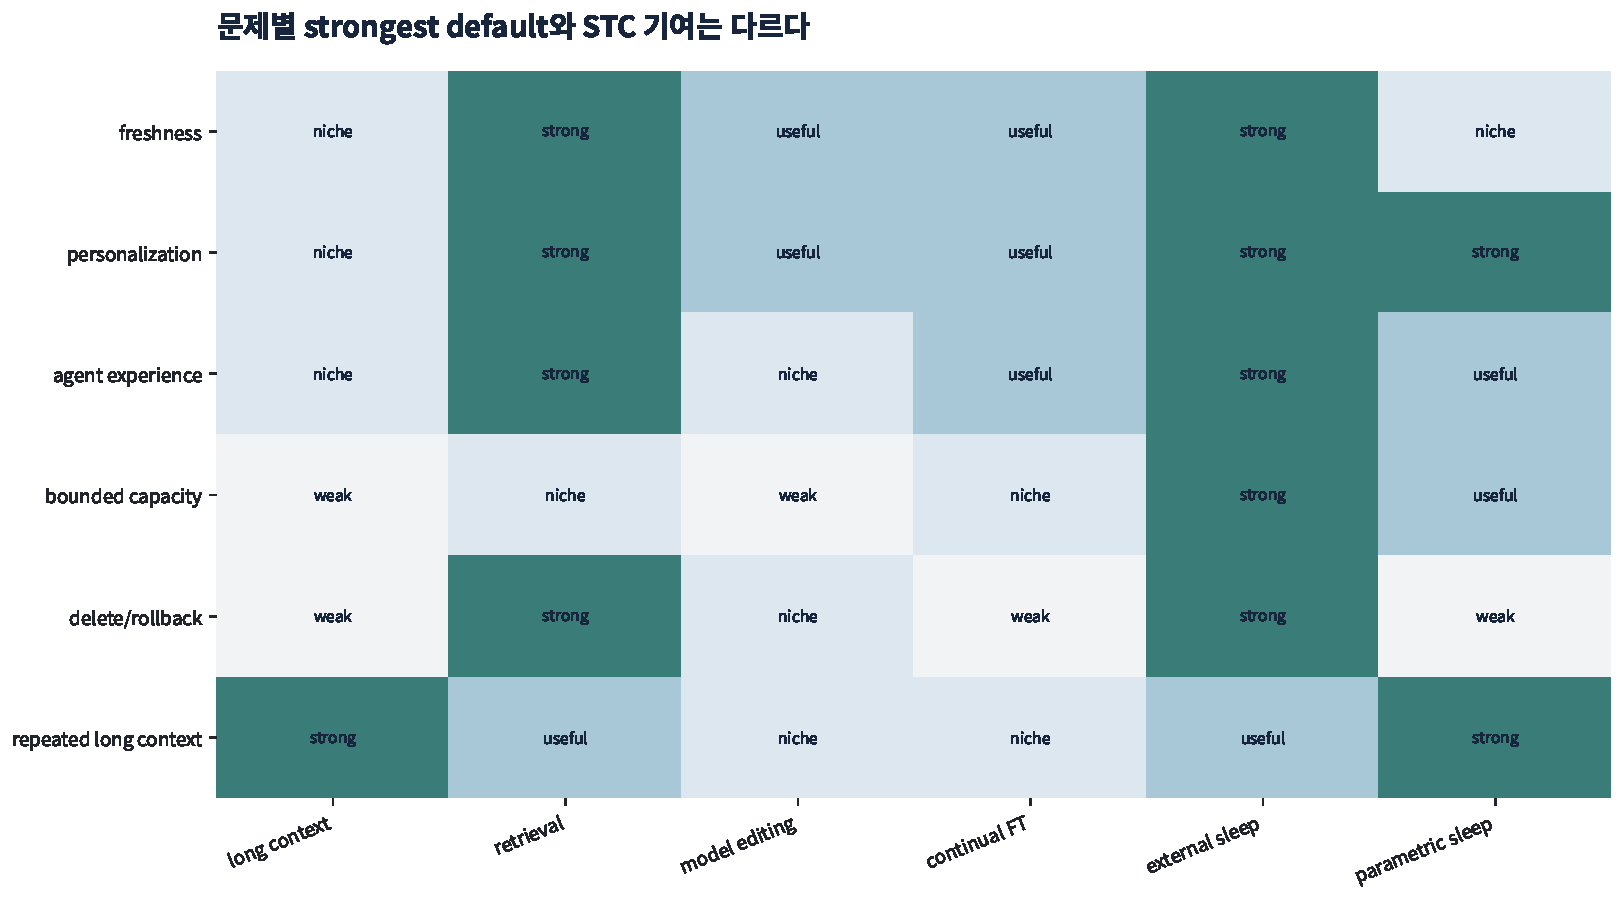
\includegraphics[width=0.96\textwidth]{figures/stc-f004.pdf}
  \caption{문제별 방법 적합도. 한 method가 모든 row에서 우세하지 않으며, external sleep과 parametric
  sleep도 서로 다른 failure surface를 가진다.}
  \stcfigure{STC-F004}
  \figsource{Original synthesis; SRC-STC-0002, SRC-STC-0031, SRC-STC-0036}{행은 freshness, personalization, agent experience, bounded capacity, deletion, repeated long context이고 열은 long context, retrieval, editing, continual FT, external sleep, parametric sleep인 색상 행렬.}
  \label{fig:problem-solution-matrix}
\end{figure}

\section{P1–P4: static deployment, personalization, experience, freshness}

\textbf{Static deployment.} Pre/post-training이 끝난 fixed model은 배포 뒤 새 사용자 분포와 도구 변화에
자동 적응하지 않는다. Strongest default는 prompt/profile retrieval과 주기적 global refresh다.
Sleep은 반복되는 local distribution을 idle window에서 정리해 다음 query의 retrieval 또는 adapter를
미리 만드는 데 기여한다. One-off interaction이면 amortization이 없다.

\textbf{Personalization.} External profile은 explicit, editable, portable하므로 첫 baseline이다. Parametric
sleep은 같은 preference가 매우 자주 재사용되고 prompt token·retrieval latency가 누적될 때 후보가 된다.
다른 user로의 leakage와 preference drift가 크면 isolated external record가 우세하다.

\textbf{Agent experience.} Agent는 성공·실패 trace에서 strategy를 추출할 수 있다. Raw transcript를
매번 long context로 넣는 대신 external strategy bank나 procedural graph로 압축하는 것이 강한 default다.
Skill이 stable하고 반복되면 distillation이나 adapter promotion을 비교한다.

\textbf{Knowledge freshness.} Mutable fact는 timestamp, supersession, citation이 필요한 external temporal
memory가 기본이다. Weight refresh는 stale fact를 지우기 어렵고 old/new fact가 composition에서 충돌할
수 있다. 실제로 sequential fact가 weights에 encoding되어도 behaviorally unreachable할 수 있으므로
retention은 parameter storage가 아니라 access와 composition으로 측정해야 한다.\claim{STC-C032}
\parencite{srcstc0036}

\section{P5–P6: continual learning과 bounded capacity}

Continual learning은 replay, regularization, gradient constraint, isolation, growth/compaction의 도움을
받지만 어느 것도 무한 retention을 보장하지 않는다. Stable skill/procedure에는 parametric integration이
유망하고, exact changing fact와 legal delete 대상에는 external representation이 유리하다.

정적 memorization capacity 실험은 sequential access, interference, governance를 포함하지 않으므로
safe continual-learning capacity를 직접 결정하지 못한다.\claim{STC-C033} \parencite{srcstc0034,srcstc0036}
Capacity는 weights의 bits뿐 아니라 replay bytes, adapter count, router fragmentation, validation time,
index latency, rollback versions의 vector budget이다.

Rate--distortion은 무엇을 어느 fidelity로 압축할지 utility--budget trade-off로 만드는 유용한 관점이지만,
제안된 frontier가 아직 agent의 보편 empirical scaling law는 아니다.\claim{STC-C034}
\parencite{srcstc0035} Future-query distortion을 reconstruction error 하나로 대체하지 말고 task utility,
provenance recovery, temporal correctness, delete granularity를 포함한다.

\section{P7–P8: latency isolation, deletion과 rollback}

Sleep의 가장 강한 system-level 이유는 expensive transformation을 current response SLA에서 분리하는
것이다. 그렇다고 반드시 별도 datacenter cluster가 필요한 것은 아니다. State가 있는 device/region에서
local sleep을 실행하면 migration을 줄일 수 있고, shared accelerator pool이 작은 job을 batch할 수도 있다.

Deletion은 source episode가 어떤 summary, vector, graph edge, training dataset, adapter에 기여했는지
lineage를 요구한다. External memory는 더 직접적이지만 poisoned record가 agent behavior를 조용히
조종할 수 있는 attack surface를 만든다. 따라서 provenance와 revocation은 부가 metadata가 아니라
설계 요구다.\claim{STC-C037} \parencite{srcstc0042}

\section{P9–P10: repeated long context와 on-device adaptation}

Long context는 원문에 대한 one-off deep reasoning에서 강하다. Sleep compilation은 context를 summary,
graph, latent/parametric state로 바꾸는 선행 비용이 있으므로 future query distribution이 예측 가능하고
reuse가 충분할 때만 이긴다. Long context를 대체하기보다 build path로 사용하고 compact state를 serve
path에서 쓰는 complement다.

On-device sleep은 privacy, intermittent connectivity, local personalization에서 expected value가 높지만
thermal, battery, write endurance, limited validation compute가 제약이다. Cloud와 device 사이에서 raw
episode 대신 provenance-preserving delta, gradient sketch, summary만 이동시키는 split도 비교 대상이다.

\section{Synthetic replay가 문제를 증폭할 때}

Generated replay를 costless fresh data로 볼 수 없다. Real-data support가 사라진 recursive training은
distribution tail을 collapse시킬 수 있다.\claim{STC-C035} \parencite{srcstc0041} 반대로 real과 synthetic
data를 적절히 누적한 조건에서 collapse는 필연이 아니므로, 중요한 변수는 synthetic 여부의 이분법보다
recursive depth와 real-data anchoring이다.\claim{STC-C036} \parencite{srcstc0069}

\begin{table}[htbp]
\centering
\caption{문제별 가장 먼저 이겨야 할 baseline과 STC의 제한된 win condition}
\label{tab:problem-baselines-short}
\small
\begin{tabularx}{\textwidth}{p{0.20\textwidth} p{0.28\textwidth} X}
\toprule
문제 & Strongest default & STC win condition \\
\midrule
freshness & temporal retrieval & 반복 query와 controlled synthesis \\
personalization & external profile & stable high reuse, reversible scope \\
agent experience & strategy memory/reflection & multi-episode compression improves later utility \\
continual skill & replay/PEFT/global refresh & cycle-level retention at bounded state \\
capacity & admit/evict/compress & marginal utility exceeds compaction/deletion cost \\
long context & long-context inference/RAG & compile cost amortized over valid reuses \\
deletion & external lineage + rebuild & parametric state remains reconstructable cache \\
\bottomrule
\end{tabularx}
\end{table}
